%%%% DOCUMENT CLASS ************************************************************
\documentclass[print,thumbmain]{src/thesis}  % uncomment for writing
%\documentclass[final]{src/thesis} % uncomment for rendering/final version

%%%% PREAMBLE ******************************************************************
%!TEX root = ../thesis.tex
\usepackage{xcolor}

%% DEEP PURPLE
% \definecolor{thumbcolor}{RGB}{200,200,200}
% \definecolor{deepcolor}{RGB}{70,25,200}
% \definecolor{titlecolor}{RGB}{120,80,235

%% MATLAB BLUE
% \definecolor{thumbcolor}{RGB}{200,200,200}
% \definecolor{deepcolor}{RGB}{0,0,0}
% \definecolor{titlecolor}{RGB}{0,114,159}

%% PRUSA ORANGE
\definecolor{thumbcolor}{RGB}{250,180,140}
\definecolor{deepcolor}{RGB}{0,0,0}
\definecolor{titlecolor}{RGB}{238,112,35}

%% SOFT ORANGE
% \definecolor{thumbcolor}{RGB}{250,180,140}
% \definecolor{deepcolor}{RGB}{0,0,0}
% \definecolor{titlecolor}{RGB}{250,180,140}

% \definecolor{C1}{RGB}{0,88,168}
% \definecolor{C2}{RGB}{202,30,4}
% \definecolor{C3}{RGB}{52,167,63}
% \definecolor{C4}{RGB}{238,112,35}

\definecolor{Matlab1}{RGB}{0,114,189}
\definecolor{Matlab2}{RGB}{217,83,25}
\definecolor{Matlab3}{RGB}{237,177,32}
\definecolor{Matlab4}{RGB}{126,47,142}
\definecolor{Matlab5}{RGB}{119,172,48}
\definecolor{Matlab6}{RGB}{77,190,238}
\definecolor{Matlab7}{RGB}{162,20,47}

\definecolor{C2}{RGB}{202,30,4}
\definecolor{C3}{RGB}{52,167,63}
\definecolor{C4}{RGB}{238,112,35}

\definecolor{magenta}{RGB}{255,20,120}
\definecolor{lightgreen}{RGB}{120,194,22}

%!TEX root = ../thesis.tex
%\usepackage{amsmath}
\usepackage[fleqn]{amsmath}
\usepackage{amsfonts}
\usepackage{amssymb}
\usepackage{accents}
\usepackage{amsthm}
\usepackage{appendix}
\usepackage{afterpage}
\usepackage{array}
\usepackage[dutch,english]{babel}
\usepackage[utf8]{inputenc}
\usepackage[autostyle]{csquotes}
\usepackage{enumitem}
\usepackage{epsfig}
\usepackage{epstopdf}
\usepackage{fancyhdr}
\usepackage{float}
\usepackage{graphicx}
\usepackage{lipsum}
\usepackage{longtable}
\usepackage{multicol}
\usepackage{multirow}
\usepackage[numbers,sort&compress]{natbib}
%\usepackage[sort&compress]{natbib}
\usepackage[final]{pdfpages}
\usepackage{relsize}
\usepackage{subfig}
\usepackage{siunitx}

\usepackage{tcolorbox}
\usepackage{thmtools}
\usepackage{todonotes}
%\usepackage{tikz}      % The tikz package is added in mrthesis.cls for producing thumbindex
\usepackage{url}
\usepackage{textcomp}

\usepackage[bookmarks=true,bookmarksopen=false,colorlinks=true,pdfpagelayout=TwoColumnRight]{hyperref}
\hypersetup{
    colorlinks,%
    citecolor=deepcolor,%
    colorlinks=true,%
    filecolor=black,%
    linkcolor=deepcolor,%
    urlcolor=thumbcolor,
    }
\usepackage{bookmark}

%\setlength{\mathindent}{1.75cm}
\setlength{\mathindent}{1.25cm}
\renewcommand{\baselinestretch}{1.05}

%!TEX root = ../thesis.tex

% Texts or
\renewcommand{\emph}[1]{'\textit{#1}'}
\newcommand{\sorotoki}{\textup{\texttt{SOROTOKI}} }
\newcommand{\matlab}{\textup{\texttt{MATLAB}} }
\newcommand{\data}[1]{(\raisebox{-2.7pt}{\textcolor{#1}{\,\Huge{\textbf{-}}}})}

% Equations/math
\newcommand{\be}{\begin{equation}}
\newcommand{\ee}{\end{equation}}
\newcommand{\benn}{\begin{equation*}}
\newcommand{\eenn}{\end{equation*}}
\newcommand{\bea}{\begin{eqnarray}}
\newcommand{\eea}{\end{eqnarray}}
\newcommand{\beann}{\begin{eqnarray*}}
\newcommand{\eeann}{\end{eqnarray*}}
\newcommand{\ba}{\begin{align}}
\newcommand{\ea}{\end{align}}
\newcommand{\bpm}{\begin{pmatrix}}
\newcommand{\epm}{\end{pmatrix}}
\newcommand{\bbm}{\begin{bmatrix}}
\newcommand{\ebm}{\end{bmatrix}}
\newcommand{\bc}{\begin{center}}
\newcommand{\ec}{\end{center}}
\newcommand{\pwr}[1]{\cdot10^{\textrm{#1}}}

% Symbols and annotations
%\newcommand{\fB}{\boldsymbol{f}}
\newcommand{\maT}{\text{ma}}
\newcommand{\qR}{\mathrm{q}}
\newcommand{\RBB}{\mathbb{R}}
\newcommand{\rmsT}{\text{rms}}
\newcommand{\uB}{\boldsymbol{u}}
\newcommand{\xBF}{\mathbf{x}}
\newcommand{\interior}{\operatorname{int}}

% Tikz figures
\newcommand{\SF}{1}                 % Scaling factor
\newcommand{\TS}{\normalsize}       % Text size
\newcommand{\lw}{0.7pt}             % Line width
\newcommand{\TSTick}{\small}        % Text size axis labels
\newcommand{\axislabels}[2]{\foreach \x/\y/\s in {#1} {\node[#2,inner sep=1mm] at (\x,\y) {\TSTick $\s$};}}
\newcommand{\wheel}[3]{ \draw[line width=\lw] (#1,#2) circle (#3);
                        \fill[bottom color=MRblue!60!black!80,top color=MRblue!10] (#1,#2) circle (#3-0.5*\lw);
                        \fill[color=MRblue!30] (#1,#2) circle (#3-\lw);
                        \fill[top color=MRblue!60!black!80,bottom color=MRblue!10] (#1,#2) circle (0.7*#3);
                        \fill[color=MRblue!30] (#1,#2) circle (0.7*#3-\lw);
                        \fill[color=black] (#1,#2) circle (0.1*#3);}

\newcommand{\CoM}[3]{\filldraw[inner color=white,outer color=black!7!white,draw=black,line width=\lw] (#1,#2) circle (#3+0.5*\lw);
                     \begin{scope}[xshift=#1,yshift=#2]
                        \clip(-#3,0) -- (0,0) -- (0,#3) -- (#3,#3) -- (#3,0) -- (0,0) -- (0,-#3) -- (-#3,-#3) -- cycle;
                        \fill[inner color=black!50!white,outer color=black] (0,0) circle (#3);
                     \end{scope}}

\definecolor{MRdarkblue}{RGB}{16,9,88}      % Define a set of colors to be used throughout thesis
\definecolor{MRred}{RGB}{152,0,0}
\definecolor{MRgreen}{RGB}{0,146,69}
\definecolor{MRblue}{RGB}{53,153,204}
\definecolor{MRorange}{RGB}{220,85,30}
\definecolor{MRlightgreen}{RGB}{217,224,33}
\definecolor{MRyellow}{RGB}{255,214,0}
\definecolor{MRgrey}{gray}{0.95}
\usetikzlibrary{arrows}
\usetikzlibrary{patterns}
\usetikzlibrary{decorations.markings}
\usetikzlibrary{shadings}
\usetikzlibrary{shapes}

% Counters
\newcounter{ContNum}        % Counter for the contributions
\renewcommand{\theContNum}{\Roman{ContNum}}

% Other
\newcommand\blankfootnote[1]{%
  \let\thefootnote\relax\footnotetext{#1}%
  \let\thefootnote\svthefootnote%
}
\newcounter{numfootnote}
\newcommand\numfootnote[1]{%
    \stepcounter{numfootnote}%
    \newcommand{\thefootnote}{\thenumfootnote}%
    \footnote{#1}
}

\newcommand{\disclaimer}{\\[\baselineskip]  A detailed list of the differences between this chapter and the article on which it is based is provided in the %\hyperref[chap: Modifications]{\emph{Modifications}}
\emph{Modifications} chapter of this thesis.}
\newcommand{\itemheader}[1]{~\\ \noindent\textbf{#1.}\ \ }
\newcommand{\itemheaderNewpage}[1]{\newpage \noindent\textbf{#1.}\ \ }
\newcommand{\contribution}[2]{\refstepcounter{ContNum}#2 \vspace*{2.1mm}\begin{tcolorbox}[colback=black!2!white,colframe=black!20!white] \textbf{Contribution \Roman{ContNum}.} {\em #1} \end{tcolorbox}\vspace*{2.1mm}}
\newcommand{\objective}[1]{\begin{tcolorbox}[colback=black!2!white,colframe=black!20!white] {\em #1} \end{tcolorbox}}
\newcommand{\terminology}[2]{\begin{tcolorbox}[colback=black!2!white,colframe=black!20!white] {\textbf{Terminology: } \textbf{#1} \em #2} \end{tcolorbox}}
\newcommand{\cover}[1]{\ifprint{}\else\includepdf[pages=-]{#1}\cleardoublepage\fi}

%!TEX root = ../thesis.tex
%%%% ***************************************************************************
%%%% VECTOR NOTATIONS **************************************************************
% base notation
\renewcommand{\vec}[1]{\boldsymbol{#1}}
\newcommand{\mat}[1]{\boldsymbol{#1}}
\newcommand{\ten}[1]{\boldsymbol{\mathcal{#1}}}

% special vectors
\newcommand{\bvec}[1]{\bar{\boldsymbol{#1}}}
\newcommand{\tvec}[1]{\widetilde{\!\boldsymbol{#1}}}
\newcommand{\tmat}[1]{\widetilde{\boldsymbol{#1}}}
\newcommand{\dmat}[1]{\dot{\!\boldsymbol{#1}}}
\newcommand{\dvec}[1]{\dot{\boldsymbol{#1}}}

% ROMAN alphabet
\newcommand{\aB}{{\vec{a}}}
\newcommand{\bB}{{\vec{b}}}
\newcommand{\cB}{{\vec{c}}}
\newcommand{\dB}{{\vec{d}}}
\newcommand{\eB}{{\vec{e}}}
\newcommand{\fB}{{\vec{f}}}
\newcommand{\gB}{{\vec{g}}}
\newcommand{\hB}{{\vec{h}}}
\newcommand{\iB}{{\vec{i}}}
\newcommand{\jB}{{\vec{j}}}
\newcommand{\kB}{{\vec{k}}}
\newcommand{\lB}{{\vec{l}}}
\newcommand{\mB}{{\vec{m}}}
\newcommand{\nB}{{\vec{n}}}
\newcommand{\pB}{{\vec{p}}}
\newcommand{\oB}{{\vec{o}}}
\newcommand{\qB}{{\vec{q}}}
\newcommand{\rB}{{\vec{r}}}
\newcommand{\sB}{{\vec{s}}}
\newcommand{\tB}{{\vec{t}}}
\newcommand{\wB}{{\vec{w}}}
\newcommand{\vB}{{\vec{v}}}
\newcommand{\xB}{{\vec{x}}}
\newcommand{\yB}{{\vec{y}}}
\newcommand{\zB}{{\vec{z}}}

% CAPITAL ROMAN alphabet
\newcommand{\AB}{{\vec{A}}}
\newcommand{\BB}{{\vec{B}}}
\newcommand{\CB}{{\vec{C}}}
\newcommand{\DB}{{\vec{D}}}
\newcommand{\EB}{{\vec{E}}}
\newcommand{\FB}{{\vec{F}}}
\newcommand{\GB}{{\vec{G}}}
\newcommand{\HB}{{\vec{H}}}
\newcommand{\IB}{{\vec{I}}}
\newcommand{\JB}{{\vec{J}}}
\newcommand{\KB}{{\vec{K}}}
\newcommand{\LB}{{\vec{L}}}
\newcommand{\MB}{{\vec{M}}}
\newcommand{\NB}{{\vec{N}}}
\newcommand{\PB}{{\vec{P}}}
\newcommand{\OB}{{\vec{O}}}
\newcommand{\QB}{{\vec{Q}}}
\newcommand{\RB}{{\vec{R}}}
\newcommand{\SB}{{\vec{S}}}
\newcommand{\TB}{{\vec{T}}}
\newcommand{\WB}{{\vec{W}}}
\newcommand{\VB}{{\vec{V}}}
\newcommand{\XB}{{\vec{X}}}
\newcommand{\YB}{{\vec{Y}}}
\newcommand{\ZB}{{\vec{Z}}}

\newcommand{\alphaB}{{\vec{\alpha}}}
\newcommand{\betaB}{{\vec{\beta}}}
\newcommand{\gammaB}{{\vec{\gamma}}}
\newcommand{\deltaB}{{\vec{\deltaB}}}
\newcommand{\epsilonB}{{\vec{\epsilonB}}}
\newcommand{\varepsilonB}{{\vec{\varepsilonB}}}
\newcommand{\xiB}{{\vec{\xi}}}
\newcommand{\PhiB}{{\vec{\Phi}}}
\newcommand{\phiB}{{\vec{\phi}}}
\newcommand{\psiB}{{\vec{\ssi}}}
\newcommand{\PsiB}{{\vec{\Psi}}}
\newcommand{\thetaB}{{\vec{\theta}}}
\newcommand{\ThetaB}{{\vec{\Theta}}}
\newcommand{\etaB}{{\vec{\eta}}}

%!TEX root = ../thesis.tex
%%%% ***************************************************************************
%%%% NOMENCLATURE **************************************************************
\usepackage{mathtools}

%%%%%%% ENTITIES %%%%%%%
\newcommand{\defas}[1]{\triangleq}
\newcommand{\grad}[1]{\nabla_{\!#1}\,}
\newcommand{\nn}{{n\times n}}

\newcommand{\ie}{\textit{i.e.}}
\newcommand{\eg}{\textit{e.g.}}
\newcommand{\blank}{\,\cdot\,}

% sets
\newcommand{\R}{\mathbb{R}}
\newcommand{\E}{\mathbb{E}}
\newcommand{\N}{\mathbb{N}}
\newcommand{\Z}{\mathbb{Z}}
\newcommand{\seg}[1]{\textup{\textrm{se}}(#1)}
\newcommand{\cose}[1]{\textup{\textrm{se}}^*(#1)}
\newcommand{\sog}[1]{\textup{\textrm{so}}(#1)}
\newcommand{\coso}[1]{\textup{\textrm{so}}^*(#1)}
\newcommand{\SO}[1]{\textup{\textrm{SO}}(#1)}
\newcommand{\SE}[1]{\textup{\textrm{SE}}(#1)}
\newcommand{\Sim}[1]{\textup{\textrm{Sim}(#1)}}
\newcommand{\atantwo}{\textup{\textrm{atan2}}}
\newcommand{\erf}{\textup{\textrm{erf}}}
\newcommand{\Id}{\text{id}}

% compact sets
\newcommand{\Rp}{\mathbb{R}_{\ge0}}
\newcommand{\Rn}{\mathbb{R}_{\le0}}
\newcommand{\Rsp}{\mathbb{R}_{>0}}
\newcommand{\Rsn}{\mathbb{R}_{<0}}
% domains
\newcommand{\Ts}{\mathbb{T}}
\newcommand{\Xs}{\mathbb{X}}
\newcommand{\Bs}{\mathbb{B}}
\newcommand{\Vs}{\mathbb{V}}
\newcommand{\Ss}{\mathbb{S}}
% functional
\newcommand{\Hm}{\mathcal{H}}
\newcommand{\La}{\mathcal{L}}
% tensors
\newcommand{\Mt}{\mathcal{M}}
\newcommand{\Ct}{\mathcal{C}}
\newcommand{\Ft}{\mathcal{F}}
\newcommand{\Uf}{\mathcal{U}}
\newcommand{\Wf}{\mathcal{W}}
\newcommand{\g}{\mathfrak{g}}
\newcommand{\Vf}{\mathcal{V}}
\newcommand{\Tf}{\mathcal{T}}
\newcommand{\Kf}{\mathcal{K}}
\newcommand{\Lf}{\mathcal{L}}

\newcommand{\p}{\partial}
\newcommand{\dt}{\Delta t}

\renewcommand{\d}{^{\raisebox{.2ex}{$\scriptscriptstyle d$}}}
\newcommand{\T}{^{\raisebox{.2ex}{$\scriptscriptstyle\top$}}}
\newcommand{\inv}{^{\raisebox{.2ex}{$\scriptscriptstyle-1$}}}
\newcommand{\pinv}{^{\raisebox{.2ex}{$\scriptscriptstyle\dagger$}}}
\newcommand{\ginv}{^{\raisebox{.2ex}{$\scriptscriptstyle+$}}}
\newcommand{\pinvt}{^{\raisebox{.2ex}{$\scriptscriptstyle+\top$}}}
%\newcommand{\grav}{^{\raisebox{.1ex}{$\scriptstyle\textrm{g}$}}}
%\newcommand{\elastic}{^{\raisebox{.1ex}{$\scriptstyle\textrm{e}$}}}
\newcommand{\grav}{_{\scriptstyle\textrm{g}}}
\newcommand{\elastic}{_{\scriptstyle\textrm{e}}}

\DeclarePairedDelimiter\ceil{\lceil}{\rceil}
\DeclarePairedDelimiter\floor{\lfloor}{\rfloor}

\renewcommand{\dim}{\text{dim}}
\newcommand{\trace}{\text{trace}}
\newcommand{\diag}[1]{\textnormal{diag}\left\{ {#1} \right\}}
\newcommand{\blkdiag}[1]{\textnormal{blkdiag}\left\{ {#1} \right\}}

\newcommand{\Q}{\mathcal{Q}}
\newcommand{\Qnc}{\vec{Q}^{\textrm{nc}}}
\newcommand{\q}{{\vec{q}}}
\newcommand{\dq}{{\dot{\vec{q}}}}
\newcommand{\ddq}{{\ddot{\vec{q}}}}
%\newcommand{\pB}{{\boldsymbol{\gamma}}}
\newcommand{\dpB}{{\dot{\boldsymbol{\gamma}}}}
\newcommand{\ddpB}{{\ddot{\boldsymbol{\gamma}}}}

%\newcommand{\MB}{\boldsymbol{M}}
%\newcommand{\CB}{\boldsymbol{C}}
%newcommand{\NB}{\boldsymbol{N}}
%\newcommand{\GB}{\boldsymbol{G}}
%\renewcommand{\fB}{\boldsymbol{f}}
%\newcommand{\JB}{\boldsymbol{J}}
\newcommand{\dJB}{\dot{\boldsymbol{J}}}

\newcommand{\ad}{\textbf{ad}}
\newcommand{\Ad}{\textbf{Ad}}
\newcommand{\rank}{\textnormal{rank}}
\newcommand{\col}{\textnormal{col}}
\newcommand{\row}{\textnormal{row}}
\newcommand{\nc}{\textnormal{nc}}

%\newcommand{\gB}{\boldsymbol{g}}
%\newcommand{\UB}{\boldsymbol{U}}
%\newcommand{\LambdaB}{\boldsymbol{\Lambda}}
%\newcommand{\GammaB}{\boldsymbol{\Gamma}}
%\newcommand{\gammaB}{\boldsymbol{\gamma}}
%\newcommand{\KappaB}{\boldsymbol{\Kappa}}
%\newcommand{\phiB}{\boldsymbol{\phi}}
%\newcommand{\sB}{\boldsymbol{\sigma}}
%\renewcommand{\pB}{\boldsymbol{p}}
%\newcommand{\dB}{\boldsymbol{d}}
\newcommand{\ddB}{\dot{\boldsymbol{d}}}
%\newcommand{\FB}{\boldsymbol{F}}
\newcommand{\dFB}{\dot{\boldsymbol{F}}}
%\newcommand{\xB}{\boldsymbol{x}}
\newcommand{\dxB}{\dot{\boldsymbol{x}}}
\newcommand{\ddxB}{\ddot{\boldsymbol{x}}}
%\newcommand{\nuB}{\boldsymbol{\nu}}
\newcommand{\PiB}{\boldsymbol{\Pi}}
\newcommand{\piB}{\boldsymbol{\pi}}
%\newcommand{\JB}{\boldsymbol{J}}
%\newcommand{\dJB}{\dot{\boldsymbol{J}}}
%\newcommand{\VB}{\boldsymbol{V}}
\newcommand{\tauB}{\boldsymbol{\tau}}

%\newcommand{\trace}[1]{\textnormal{trace}\left( {#1} \right)}
\renewcommand{\det}[1]{\textnormal{det}\left( {#1} \right)}
\newcommand{\inner}[2]{ \langle {#1}, {#2} \rangle}
\newcommand{\subto}{\;\textrm{s.t.}\;}
\newcommand{\config}[1]{{#1}^\circ}

%!TEX root = ../thesis.tex
% Theorems, remarks, propositions, etc.
\declaretheorem[name={Remark},style=plain,numberwithin=chapter]{rmk}
\declaretheorem[name={Definition},style=definition,numberwithin=chapter]{dfn}
\declaretheorem[name={Theorem},qed=$\blacktriangle$,style=plain,numberwithin=chapter]{thm}
\declaretheorem[name={Lemma},qed=$\blacktriangle$,style=plain,numberwithin=chapter]{lem}
\declaretheorem[name={Assumption},style=definition,numberwithin=chapter]{asm}
\declaretheorem[name={Property},style=plain,numberwithin=chapter]{prop}
\declaretheorem[name={Example},style=plain,numberwithin=chapter]{example}
\declaretheorem[name={Corollary},qed=$\blacktriangle$,style=plain,numberwithin=chapter]{cor}
\declaretheorem[name={Intermezzo},style=definition,numberwithin=chapter]{intermez}

%!TEX root = ../thesis.tex
\newif\ifistoreview
\istoreviewtrue

\newcommand{\setreviewson}{\istoreviewtrue}
\newcommand{\setreviewsoff}{\istoreviewfalse}

\RequirePackage{soul}
\RequirePackage{xcolor}
\RequirePackage{todonotes}

\definecolor{aoenglish}{rgb}{0.95,0.9,1}

\newcommand{\alertColor}{\textcolor{red}}
\newcommand{\removeColor}{\textcolor{red}}
\newcommand{\addColor}{\textcolor{titlecolor}}
\newcommand{\writeColor}{\textcolor{aoenglish}}

\newcommand{\alert}[1]{\ifistoreview\alertColor{#1}\else #1\fi}
\newcommand{\rewritten}[1]{\ifistoreview\writeColor{#1}\else #1\fi}
\newcommand{\remove}[1]{\ifistoreview\alertColor{\st{#1}}\else #1\fi}
\newcommand{\add}[1]{\ifistoreview\addColor{#1}\else #1\fi}
\newcommand{\substitute}[2]{\ifistoreview\remove{#1}~\add{#2} \else #1\fi}
\newcommand{\replace}[2]{\ifistoreview\remove{#1}~\add{#2}\else #1\fi}
\newcommand{\highlight}[1]{\hl{#1}}

\newcommand{\commentary}[2]{\highlight{#1}\todo[inline]{#2}}
\sethlcolor{aoenglish}

%!TEX root = ../thesis.tex
\usepackage{tikz}
\usepackage{pgfplots}
% and optionally (as of Pgfplots 1.3):
\pgfplotsset{compat=newest}
\pgfplotsset{plot coordinates/math parser=false}
\newlength\figureheight
\newlength\figurewidth

%\usepackage{tikz}
%\usepackage{pgfplots}
\usepackage{pgfgantt}
\usepackage{pdflscape}
\pgfplotsset{compat=newest}
\pgfplotsset{plot coordinates/math parser=false}
%\setlength\fwidth{0.5\textwidth}
% \usepackage[outline]{contour} % glow around text
% \usepackage{pgfplots}
% \usepackage{grffile}
% \usepackage{amsmath}
% \usepackage[utf8]{inputenc}
% \usepackage{pgfgantt}
% \usepackage{pdflscape}
%
% \usetikzlibrary{calc}
% \usetikzlibrary{intersections}
% \usetikzlibrary{decorations.markings}
% \usetikzlibrary{fadings}
% \usetikzlibrary{angles,quotes} % for pic (angle labels)
% \usetikzlibrary{decorations.pathreplacing} % for curly braces
% \tikzset{>=latex} % for LaTeX arrow head
% \contourlength{1.7pt}
% \pgfplotsset{compat=newest}
% %\pgfplotsset{compat = 1.3}
% %% the following commands are needed for some matlab2tikz features
\usetikzlibrary{plotmarks}
\usetikzlibrary{arrows.meta}
\usepgfplotslibrary{patchplots}

% \colorlet{myblue}{blue!80!black}
% \colorlet{myred}{black!50!red}
% \colorlet{watercol}{blue!70!cyan!50}
% \tikzstyle{myarr}=[-{Latex[length=3,width=2]}]
% \tikzstyle{water}=[ball color=watercol]
%
% \tikzset{
%   beam/.style={very thick,line cap=round,line join=round},
% }


%%%% Graphics paths
% **********************************************************
\graphicspath{{img/}{../../img/}{../../../img/}}

%%%% REVIEWING OF THESIS
% **********************************************************
%\usepackage{showframe}
\setreviewsoff

%%%% DOCUMENT COLORS  **********************************************************
% see src/colors to change colors

%%%% DOCUMENT DETAILS **********************************************************
\author{Name of Author}
\newcommand{\placeofbirth}{Place of birth}
\renewcommand{\year}{2022}
\newcommand{\defensedate}{maandag 30 december 2022}
\newcommand{\defensetime}{16:00}
\newcommand{\maintitle}{Awesome thesis title}
\newcommand{\subtitle}{with an awesome subtitle}
\newcommand{\isbn}{123-45-678-9012-3}     % 123boldmath-45-678-9012-3
\newcommand{\printer}{Name of printer || www.printerswebsite.nl}
\newcommand{\rector}{prof. dr. REctor}
% other relevant meta data about the thesis can be found in preface.tex

\makeatletter % generates all the \author stuff
%%%% MAIN DOCUMENT *************************************************************
\begin{document} %%%%%%%%%%%%%%%%%%%%%%%%%%%%%%%%%%%%%%%%%%%%%%%%%%%%%%%%%%%%%%%
%%%% ***************************************************************************
\pagenumbering{roman}
\thispagestyle{empty}

%%%% FRONT MATTERS *************************************************************
\cover{thesis_front.pdf}    % Adds your thesis' front cover if the option 'print' is NOT used. Printing companies require the thesis cover to be supplied separately and in a different format. Definition of \cover{} is given in commands.tex.

% Front matter
%!TEX root = ../thesis.tex
% First page
\thispagestyle{empty}
\vspace*{30mm}\noindent
\begin{center}
{\LARGE\sf\maintitle}\\[4.5cm] %\\[7mm]
{\Large\sf \@author}
\end{center}

\newpage
\thispagestyle{empty}

% Page with c logo etc.
\vspace*{\fill}

\hspace*{-7mm}
\includegraphics[width=6cm]{TUeLOG_new.eps}\\
{\small The work described in this thesis was carried out at the Eindhoven University of
Technology.}\\[8mm]

\hspace*{-4mm}
\includegraphics[width=2.5cm]{disc_logo_kleur.png}\\[2mm]
\noindent\bgroup\small
The research reported in this thesis is part of the research program of the Dutch Institute of Systems and Control (DISC). The author has successfully completed the educational program of the Graduate School DISC.
\\[8mm]

\noindent\bgroup\small
A catalogue record is available from the Eindhoven University of Technology Library.\\
ISBN: \isbn\\[4mm]
Typeset by the author using the pdf \LaTeX \ documentation system.\\
Cover design: Name of cover designer \\
Reproduction: \printer\\[8mm]
\copyright\year by \@author. All rights reserved.}
\egroup

\newpage
\thispagestyle{empty}


% Title page

\vspace*{30mm}
\begin{center}
{\LARGE\sf\maintitle}\\[30mm] %\\[7mm]
{\large\textsc{Proefschrift}}\\[8mm]
ter verkrijging van de graad van doctor aan de\\
Technische Universiteit Eindhoven, op gezag van de\\
rector magnificus \rector, voor een\\
commissie aangewezen door het College voor\\
Promoties, in het openbaar te verdedigen\\
op \defensedate\ om \defensetime\ uur\\[8mm]
door\\[8mm]
\@author\\[8mm]
geboren te \placeofbirth
\end{center}
\vfill

\newpage
\thispagestyle{empty}

\noindent
Dit proefschrift is goedgekeurd door de promotoren en de samenstelling van de promotiecommissie is als volgt:\\[7mm]

\noindent
\begin{tabular}{@{}l p{9.8cm}}
voorzitter:                 &   prof. dr. xx. xxxxxxxxx \\                \\
promotor:                   &   prof. dr. xx. xxxxxxxxx \\
co-promotor:                &   prof. dr. xx. xxxxxxxxx \\
leden:                      &   prof. dr. xx. xxxxxxxxx \\
                            &   prof. dr. xx. xxxxxxxxx \\
                            &   dr. xx. xxxxxxxxx \\
                            &   dr. xx. xxxxxxxxx \\
\end{tabular}

\vfill
\noindent
Het onderzoek dat in dit proefschrift wordt beschreven is uitgevoerd in overeenstemming met de TU/e Gedragscode Wetenschapsbeoefening.

%*********************************************************************************%
\chapter*{Summary} % Try to keep within approx 350 words / one page
\addcontentsline{toc}{chapter}{Summary}
\markboth{Summary}{Summary}


\begin{center}
\rule{\textwidth}{.75pt}\vspace*{1mm}
\textbf{{\Large State Your Thesis Title Here\\[2mm] With a Linebreak if Needed}}
\rule{\textwidth}{.75pt}
\end{center}
\vspace*{2ex}


\lipsum[1-4]

\vspace*{11pt}\noindent
\textbf{Keywords:} \ \ Keyword 1, Keyword 2, Keyword 3, ...

%*********************************************************************************%
\chapter*{Samenvatting}
\addcontentsline{toc}{chapter}{Samenvatting}
\markboth{Samenvatting}{Samenvatting}

IN DUTCH:
\lipsum[1-4]


\vspace*{11pt}\noindent
\textbf{Trefwoorden:} \ \ Trefwoord 1, Trefwoord 2, Trefwoord 3, ...


%*********************************************************************************%
\chapter*{Societal summary}
\addcontentsline{toc}{chapter}{Societal summary}
\markboth{Societal summary}{Societal summary}

%*********************************************************************************%
% FROM "Information for Doctoral candidates"
%*********************************************************************************%

%Writing a public summary is part of the completion of PhD-projects at TU/e since 2017. It serves to open up the results of PhD-research to larger audiences, among which journalists and the general audience.

%The doctoral candidate writes the public summary of
%maximum 600 words
%before submitting form 2. Guidelines, examples and a template for writing a public summary can be found at www.tue.nl/promoties. The candidate sends the summary to the science information officers of CEC, via the upload form on the Promotions website. They will contact the doctoral candidate in order to jointly do editing, if necessary, and make sure the text is comprehensible and accessible.

%The final version of the summary will be published on the TU/e website, in the overview of PhD defenses. CEC draws the attention of journalists to this overview, and targets journalists directly with summaries. The summary will also be available online via the library.

%It is helpful if the candidate also supplies a picture, via the upload form. This may be a picture of the candidate, or a crucial part or result of the research. The picture will be included in the online overview of PhD’s, in landscape orientation and in quite small size. Therefore the content of the picture should be recognizable even in small size.
%Writing a public summary is not a prerequisite for graduation, but the university appreciates it very much if you do write one. In the department of Mechanical Engineering however the public summary (a.k.a. societal summary) is obligatory.

%*********************************************************************************%

IN ENGLISH:
\lipsum[5-9]

%%%% NOMENCLATURE **************************************************************
\cleardoublepage
\pdfbookmark{\contentsname}{Contents}
\tableofcontents

\newpage
\newenvironment{Nomen}
    {\vspace*{-3mm}\begin{center}
    \begin{longtable}{p{.1\textwidth} p{.83\textwidth}}
    }
    {
    \end{longtable}
    \end{center}\vspace*{-1.2cm}
    }
\newcommand{\AddSymbol}[2]{#1 & #2 \\}




%*********************************************************************************%
\chapter*{Nomenclature}
\addcontentsline{toc}{chapter}{Nomenclature}
\markboth{Nomenclature}{Nomenclature}

%*********************************************************************************%

\section*{Greek symbols}

\begin{Nomen}
\AddSymbol{$\alpha$}{What $\alpha$ is}
\AddSymbol{$\beta$}{What $\beta$ is}
\AddSymbol{$\gamma$}{What $\gamma$ is}
\AddSymbol{$\delta$}{What $\delta$ is}
\end{Nomen}


%*********************************************************************************%
\section*{Roman symbols}

\begin{Nomen}
\AddSymbol{$a$}{Description of $a$}
\AddSymbol{$b$}{Description of $b$}
\AddSymbol{$C$}{Description of $C$}
\AddSymbol{$D_a$}{Description of $D_a$}
\end{Nomen}


%*********************************************************************************%
\section*{Sub- and superscripts}

\begin{Nomen}
\AddSymbol{$\dot{(\cdot)}$}{First time derivative}
\AddSymbol{$\ddot{(\cdot)}$}{Second time derivative}
\AddSymbol{$\hat{(\cdot)}$}{Explain the reader what this means}
\AddSymbol{$(\cdot)_0$}{Explain the reader what this means}
\end{Nomen}


%*********************************************************************************%
\section*{Acronyms}

\begin{Nomen}
\AddSymbol{CoM}{Center of mass}
\AddSymbol{CoR}{Coefficient of restitution}
\end{Nomen}


%*********************************************************************************%
%\newpage
\section*{Operators and letter-like symbols}

\begin{Nomen}
\AddSymbol{$\emptyset$}{Empty set}
\AddSymbol{$\partial$}{Boundary of a set}
\AddSymbol{$\interior$}{Interior of a set}
\AddSymbol{$\sup_t$}{Supremum over continuous time $t$}
\AddSymbol{$\|\cdot\|_\maT$}{Mean absolute norm}
\AddSymbol{$\|\cdot\|_\rmsT$}{Root-mean-square norm}
\end{Nomen}

%\thispagestyle{empty}


%%%% MAIN MATTERS *************************************************************
% This state variable is used for creating the thumb index by indicating that
% the following chapter is numbered (i.e. not \chapter*{})
\isstarredchapterfalse
\cleardoublepage
\thispagestyle{empty}
\setcounter{page}{1}
\pagenumbering{arabic}
\part{Background}\label{part: intro}
\chapter{Introduction}
\label{chap: intro}
%\thispagestyle{empty}
\setcounter{page}{1}
\pagenumbering{arabic}


\vspace*{-2mm}
\section{Name of first section}
\label{sec: chap1 motivation}

\lipsum[9-13]


\section{Name of second section}
\label{sec: chap1 background}

\lipsum[14-18]

\subsection{Name of subsection}
\label{subsec: chap1 background2}

\renewcommand{\SF}{0.85}    % This 'scaling factor' is used to change the size of the image below without having to change the elements of the tikz picture
\begin{figure}[b]
    \centering
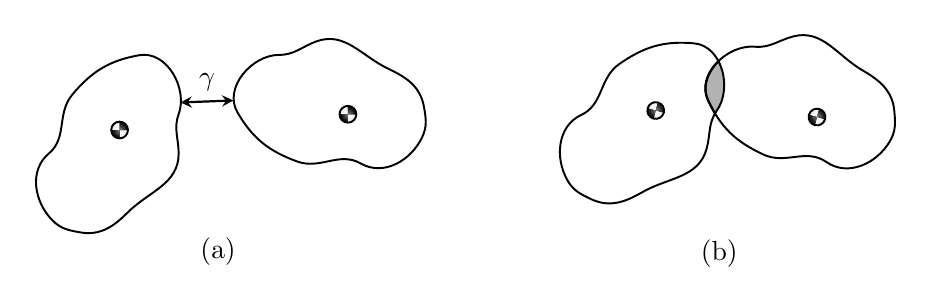
\begin{tikzpicture}[scale=\SF]
    \begin{scope}[scale=0.5]
        \draw[black,line width=0.7pt] (-1.2,1) to[out=50,in=190] (0.5,2) to[out=10,in=70] (1.5,0.5)
        to[out=-110,in=90] (1.5,-0.5) to[out=-90,in=45] (0.2,-2) to[out=-135,in=-10] (-1,-2.5) to[out=170,in=-45] (-1.7,-2.2) to[out=135,in=-140] (-1.8,-0.5) to[out=40,in=-130] (-1.2,1);
        \CoM{0}{0.1cm}{2mm};

        \draw[rotate=110,xshift=-1cm,yshift=-5cm,black,line width=0.7pt] (-1.2,1) to[out=50,in=190] (0.5,2) to[out=10,in=70] (1.5,0.5)
        to[out=-110,in=90] (1.5,-0.5) to[out=-90,in=45] (0.2,-2) to[out=-135,in=-10] (-1,-2.5) to[out=170,in=-45] (-1.7,-2.2) to[out=135,in=-140] (-1.8,-0.5) to[out=40,in=-130] (-1.2,1);
        \CoM{5.8cm}{0.5cm}{2mm};

        \draw[>=stealth,<->,thick] (1.55,0.8) -- node[pos=0.5,above]{\TS $\gamma$} (2.89,0.85);
        \draw (2.5,-3) node{\TS (a)};
    \end{scope}

    \begin{scope}[rotate=-15,scale=0.5,xshift=13cm,yshift=4cm]
        \begin{scope}
            \clip (-1.2,1) to[out=50,in=190] (0.5,2) to[out=10,in=70] (1.5,0.5)
        to[out=-110,in=90] (1.5,-0.5) to[out=-90,in=45] (0.2,-2) to[out=-135,in=-10] (-1,-2.5) to[out=170,in=-45] (-1.7,-2.2) to[out=135,in=-140] (-1.8,-0.5) to[out=40,in=-130] (-1.2,1);
            \filldraw[rotate=120,xshift=-0.5cm,yshift=-3.4cm,fill=black!30,draw=black,thick] (-1.2,1) to[out=50,in=190] (0.5,2) to[out=10,in=70] (1.5,0.5) to[out=-110,in=90] (1.5,-0.5) to[out=-90,in=45] (0.2,-2) to[out=-135,in=-10] (-1,-2.5) to[out=170,in=-45] (-1.7,-2.2) to[out=135,in=-140] (-1.8,-0.5) to[out=40,in=-130] (-1.2,1);
        \end{scope}

        \draw[black,line width=0.7pt] (-1.2,1) to[out=50,in=190] (0.5,2) to[out=10,in=70] (1.5,0.5)
        to[out=-110,in=90] (1.5,-0.5) to[out=-90,in=45] (0.2,-2) to[out=-135,in=-10] (-1,-2.5) to[out=170,in=-45] (-1.7,-2.2) to[out=135,in=-140] (-1.8,-0.5) to[out=40,in=-130] (-1.2,1);
        \CoM{0}{0.1cm}{2mm};

        \draw[rotate=120,xshift=-0.5cm,yshift=-3.4cm,black,line width=0.7pt] (-1.2,1) to[out=50,in=190] (0.5,2) to[out=10,in=70] (1.5,0.5)
        to[out=-110,in=90] (1.5,-0.5) to[out=-90,in=45] (0.2,-2) to[out=-135,in=-10] (-1,-2.5) to[out=170,in=-45] (-1.7,-2.2) to[out=135,in=-140] (-1.8,-0.5) to[out=40,in=-130] (-1.2,1);
        \CoM{4cm}{1cm}{2mm};

        \draw (2.5,-3) node{\TS (b)};
    \end{scope}
\end{tikzpicture}
\caption{This is the current style and layout of a figure caption.}
    \label{fig: chap1 impact bodies}
\end{figure}

\lipsum[19-23]


\subsection{Name of second subsection}
\label{subsec: chap1 background3}

\lipsum[1-5]

%\newpage
\section{Problem statement}
\label{sec: chap1 prob statement}

\lipsum[6-8]
Summarizing, the objective of the research is:
\vspace*{3mm}
\objective{State the objective of your PhD research here.}


\section{Research challenges and contributions}
\label{sec: chap1 contributions}

In this section, the research problem is divided in ... research challenges with the topics: topic 1, topic 2, topic 3, ... . Per research challenge, a contribution of this thesis addressing the subproblem is presented.

%**********************************************************************%

\itemheader{Topic 1}
\lipsum[1-2] This leads to the first contribution of our work:

\contribution{First contribution of your work.}{\label{contr: contribution 1}}

Explain a bit more about your first contribution.

%**********************************************************************%

\itemheader{Topic 2}
\lipsum[4-5] This leads to the second contribution of our work:

\contribution{Second contribution of your work.}{\label{contr: contribution 2}}

Explain a bit more about your second contribution.

%**********************************************************************%

\itemheader{Topic 3}
\lipsum[1-2] The last contribution of the research thus is:

\contribution{Third contribution of your work.}{\label{contr: contribution 3}}

Explain a bit more about your third contribution.


\section{Outline of the thesis}
\label{sec: chap1 outline}

\lipsum[10-12]

\itemheaderNewpage{A note for the reader} Chapters~...-... are all based on submitted/published articles and consequently are self-contained and can be read independently. A reference to the corresponding research paper is included at the beginning of each chapter.
An overview of how the chapters of this thesis relate to the contributions presented in Section~\ref{sec: chap1 contributions} is given in Table~...


% *************************************************************
%%%% first part
\cleardoublepage
\part{Second chapter}\label{part: design}
\chapter[Title of your chapter here]{Title of your chapter here}
\label{chap: chapter 1}

\blankfootnote{This chapter is based on:\\ write down the citation of the paper you are referring to in full.\disclaimer}

\chapterabstract{\lipsum[1]}

\section{Introduction}
\label{sec: chap2 intro}

\lipsum[5-7] \cite{Goebel2012}.


%%%%%%%%%%%%%%%%%%%%%%%%%%%%%%%%%%%%%%%%%%%%%%%%%%%%%%%%%%%%%%%%%%%%%%%%%%%%%%%%
\section{Section header}
\label{sec: chap2 section header}

Here's an equation:
\be
\label{eq: chap2 vector field} \dot{\xBF} = \fB(\xBF,\uB,t)
\ee
with $\uB\in\RBB^m$ the input, $t_0$ the initial time, and $t_f$ the final time. 
And below another beautiful image.

\renewcommand{\SF}{0.8}
\begin{figure}
    \centering
    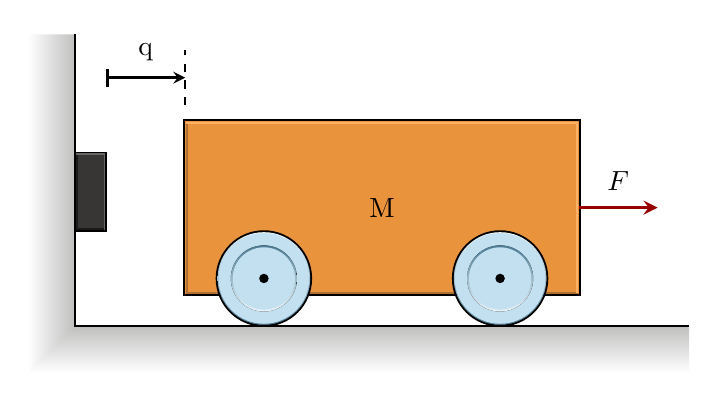
\begin{tikzpicture}[scale=\SF]
        % Fixed world
        \shade[right color=brown!2!gray!50,left color=white] (-1.2,2.7) -- (-0.6,2.7) -- (-0.6,-1) -- (-1.2,-1.6) -- cycle;
        \shade[top color=brown!2!gray!50,bottom color=white] (-0.6,-1) -- (7.2,-1) -- (7.2,-1.6) -- (-1.2,-1.6) -- cycle;
        \draw[line width=\lw] (-0.6,2.7) -- (-0.6,-1) -- (7.2,-1);

        % Stop
        \filldraw[draw=black,fill=brown!3!black!80,line width=\lw] (-0.6,0.2) rectangle (-0.2,1.2);
        \draw[color=black!90,line width=\lw] (-0.6cm+\lw,1.2cm-0.5*\lw) -- (-0.6cm+\lw,0.2cm+\lw) -- (-0.2cm-0.5*\lw,0.2cm+\lw);
        \draw[color=black!60,line width=\lw] (-0.6cm+0.5*\lw,1.2cm-\lw) -- (-0.2cm-\lw,1.2cm-\lw) -- (-0.2cm-\lw,0.2cm+0.5*\lw);

        % Cart
        \begin{scope}[xshift=0.3cm]
            \filldraw[draw=black,fill=orange!60!brown!85,line width=\lw] (0.5cm-0.5*\lw,-0.6cm-0.5*\lw) rectangle (5.5cm+0.5*\lw,1.6cm+0.5*\lw);
            \draw[color=orange!60!black!80,line width=\lw] (0.5cm+0.75*\lw,1.6cm-0.5*\lw) -- (0.5cm+0.75*\lw,-0.6cm+0.75*\lw) -- (5.5cm-0.5*\lw,-0.6cm+0.75*\lw);
            \draw[color=orange!60,line width=\lw] (0.5cm+0.5*\lw,1.6cm-\lw) -- (5.5cm-\lw,1.6cm-\lw) -- (5.5cm-\lw,-0.6cm+0.5*\lw);
            \wheel{1.5cm}{-0.4cm}{0.6cm}
            \wheel{4.5cm}{-0.4cm}{0.6cm}
        \end{scope}

        % Annotations
        \draw[dashed,line width=\lw] (0.8,1.8) -- (0.8,2.5);
        \draw[|->,>=stealth,line width=1.25*\lw] (-0.2,2.15) -- node[black,pos=0.5,above,inner sep=2mm]{\TS $\qR$} (0.8,2.15);
        \draw[->,>=stealth,line width=1.75*\lw,MRred] (5.8,0.5) -- node[black,pos=0.5,above,inner sep=2mm]{\TS $F$} (6.8,0.5);
        \draw (3.3,0.5) node[black]{\TS $\mathrm{M}$};
    \end{tikzpicture}
    \caption{Schematic representation of a controlled bouncing mass.}
    \label{fig: chap2 cntrld mass}
\end{figure}


%%%%%%%%%%%%%%%%%%%%%%%%%%%%%%%%%%%%%%%%%%%%%%%%%%%%%%%%%%%%%%%%%%%%%%%%%%%%%%%%
\section{Conclusions and discussion}
\label{sec: chap2 conclusion}

\lipsum[10-13]




% *************************************************************
%%%% second part
\cleardoublepage
\part{Third part}\label{part: design}
\chapter[Title of your chapter here]{Title of your chapter here}
\label{chap: chapter 1}

\blankfootnote{This chapter is based on:\\ write down the citation of the paper you are referring to in full.\disclaimer}

\chapterabstract{\lipsum[1]}

\section{Introduction}
\label{sec: chap2 intro}

\lipsum[5-7] \cite{Goebel2012}.


%%%%%%%%%%%%%%%%%%%%%%%%%%%%%%%%%%%%%%%%%%%%%%%%%%%%%%%%%%%%%%%%%%%%%%%%%%%%%%%%
\section{Section header}
\label{sec: chap2 section header}

Here's an equation:
\be
\label{eq: chap2 vector field} \dot{\xBF} = \fB(\xBF,\uB,t)
\ee
with $\uB\in\RBB^m$ the input, $t_0$ the initial time, and $t_f$ the final time. 
And below another beautiful image.

\renewcommand{\SF}{0.8}
\begin{figure}
    \centering
    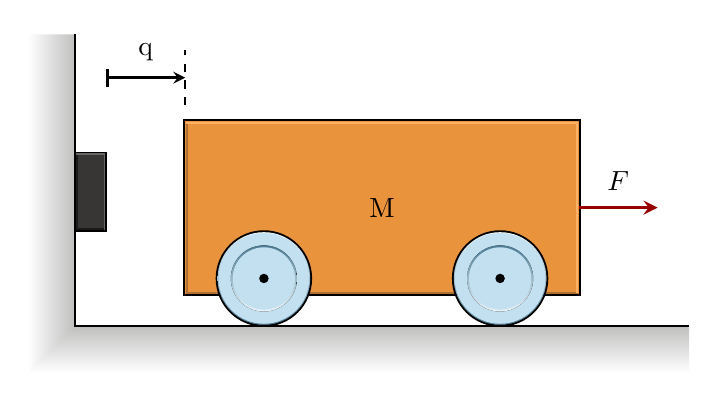
\begin{tikzpicture}[scale=\SF]
        % Fixed world
        \shade[right color=brown!2!gray!50,left color=white] (-1.2,2.7) -- (-0.6,2.7) -- (-0.6,-1) -- (-1.2,-1.6) -- cycle;
        \shade[top color=brown!2!gray!50,bottom color=white] (-0.6,-1) -- (7.2,-1) -- (7.2,-1.6) -- (-1.2,-1.6) -- cycle;
        \draw[line width=\lw] (-0.6,2.7) -- (-0.6,-1) -- (7.2,-1);

        % Stop
        \filldraw[draw=black,fill=brown!3!black!80,line width=\lw] (-0.6,0.2) rectangle (-0.2,1.2);
        \draw[color=black!90,line width=\lw] (-0.6cm+\lw,1.2cm-0.5*\lw) -- (-0.6cm+\lw,0.2cm+\lw) -- (-0.2cm-0.5*\lw,0.2cm+\lw);
        \draw[color=black!60,line width=\lw] (-0.6cm+0.5*\lw,1.2cm-\lw) -- (-0.2cm-\lw,1.2cm-\lw) -- (-0.2cm-\lw,0.2cm+0.5*\lw);

        % Cart
        \begin{scope}[xshift=0.3cm]
            \filldraw[draw=black,fill=orange!60!brown!85,line width=\lw] (0.5cm-0.5*\lw,-0.6cm-0.5*\lw) rectangle (5.5cm+0.5*\lw,1.6cm+0.5*\lw);
            \draw[color=orange!60!black!80,line width=\lw] (0.5cm+0.75*\lw,1.6cm-0.5*\lw) -- (0.5cm+0.75*\lw,-0.6cm+0.75*\lw) -- (5.5cm-0.5*\lw,-0.6cm+0.75*\lw);
            \draw[color=orange!60,line width=\lw] (0.5cm+0.5*\lw,1.6cm-\lw) -- (5.5cm-\lw,1.6cm-\lw) -- (5.5cm-\lw,-0.6cm+0.5*\lw);
            \wheel{1.5cm}{-0.4cm}{0.6cm}
            \wheel{4.5cm}{-0.4cm}{0.6cm}
        \end{scope}

        % Annotations
        \draw[dashed,line width=\lw] (0.8,1.8) -- (0.8,2.5);
        \draw[|->,>=stealth,line width=1.25*\lw] (-0.2,2.15) -- node[black,pos=0.5,above,inner sep=2mm]{\TS $\qR$} (0.8,2.15);
        \draw[->,>=stealth,line width=1.75*\lw,MRred] (5.8,0.5) -- node[black,pos=0.5,above,inner sep=2mm]{\TS $F$} (6.8,0.5);
        \draw (3.3,0.5) node[black]{\TS $\mathrm{M}$};
    \end{tikzpicture}
    \caption{Schematic representation of a controlled bouncing mass.}
    \label{fig: chap2 cntrld mass}
\end{figure}


%%%%%%%%%%%%%%%%%%%%%%%%%%%%%%%%%%%%%%%%%%%%%%%%%%%%%%%%%%%%%%%%%%%%%%%%%%%%%%%%
\section{Conclusions and discussion}
\label{sec: chap2 conclusion}

\lipsum[10-13]




% *************************************************************
\part{Closing}\label{part: closing}
\chapter{Conclusions and recommendations}
\label{chap: conclusions}
\thispagestyle{empty}

\section{Conclusions}

\lipsum[20-23]
Restate your thesis objective.

\vspace*{3mm}
\objective{State the objective of your PhD research here.}



%**********************************************************************%


\section{Recommendations}

\lipsum[1-4]

%%%% APPENDIX ******************************************************************
\appendix
\cleardoublepage
\part{Appendices}

\definecolor{thumbcolor}{gray}{0.4}     % Change the color of the thumb index tags to gray
\chapter{Appendix name}
\label{app: appendix 1}

\section{Section header}

\lipsum[1-4]

%%%% BACK MATTER ***************************************************************
\isstarredchaptertrue           % This state variable is used for creating the thumb index by indicating that the following chapter is not numbered (i.e. \chapter*{})
\bookmarksetup{startatroot}
\addtocontents{toc}{\bigskip}%
%!TEX root = ../thesis.tex
%\footnotesize
{\fontsize{9pt}{10pt}\selectfont

\bibliographystyle{ieeetr}
%\bibliographystyle{apalike}
\cleardoublepage
\phantomsection
\addcontentsline{toc}{chapter}{\bibname}
\bibliography{5_bibliography/MyBib}
%
}

\normalsize

%*********************************************************************************%
\chapter*{Acknowledgements}
\addcontentsline{toc}{chapter}{Acknowledgements}
\markboth{Acknowledgements}{Acknowledgements}




\newpage
%!TEX root = ../thesis.tex
%*********************************************************************************%
\chapter*{List of publications}
\addcontentsline{toc}{chapter}{List of publications}
\markboth{List of publications}{List of publications}
\newcommand{\ipj}{(\textit{in preparation for journal submission})}
\newcommand{\cur}{(\textit{under review})}
\newcommand{\sbm}{(\textit{submitted})}
\newcommand{\acp}{(\textit{accepted})}
\newcommand{\inp}{(\textit{in press})}
% \section*{Preliminary titles}
% \begin{enumerate}[leftmargin=2.5mm]
% \item A Control-oriented Perspective on Design and Modeling of Soft Robotic Systems;
% \item Towards a Unified Framework for Design and Model-based Control of Soft Robots;
% \item Addressing the Open Challenges in Soft Robotics: from Design to Model-based Control
% \item Design and Control Strategies for Soft Robotic Systems;
% \item Design, Modeling, Simulation and Control of Soft Robots.
% \item Design, Modeling and Control Strategies for Soft Robotics Systems;
% \item (Soft Manipulators/Soft Robotic Manipulators?)
% \end{enumerate}
%
% \section*{Preliminary committee members}
% \begin{itemize}[leftmargin=4mm]
% \item prof. J. den Toonder (TU/e, Microsystems, ICMS) \vspace{-2mm}
% \item dr. R. Luttge (TU/e, Microsystems) - Backup for Jaap \\ ............................................................................................... \vspace{-2mm}
% \item prof. G. Krijnen (Twente University) Technologies) \vspace{-2mm}
% \item prof. C.C.L. Wang (Delft University) \vspace{-2mm} \href{https://ieeexplore.ieee.org/document/9426391}{[1]}, \href{https://www.researchgate.net/publication/347965436_Jacobian-based_learning_for_inverse_kinematics_of_soft_robots}{[2]}
% \item prof R. Carloni (Rijksuniversiteit
% Groningen) - backup for Gijs \\ ............................................................................................... \vspace{-2mm}
% \item dr. E. Franco (Enrico, Imperial College London) \vspace{-2mm} \href{https://link.springer.com/article/10.1007/s11071-021-06817-1}{[1]}, \href{https://ieeexplore.ieee.org/document/9638969}{[2]}
% \item prof. H. Mochiyama (University of Tsukuba) \href{https://www.sciencedirect.com/science/article/pii/S2405896320328226?via%3Dihub}{[1]}, \href{https://ieeexplore.ieee.org/document/1242160}{[2]} \vspace{-2mm}
% \item dr. C. Duriez (INRIA Lille) \href{https://hal.inria.fr/hal-01370347/document}{[1]},\href{https://hal.archives-ouvertes.fr/hal-03192168/document}{[2]}\vspace{-2mm}
% \item prof. R. Katzschmann (ETH Zurich) \href{https://www.liebertpub.com/doi/pdfplus/10.1089/soro.2014.0022}{[1]},\href{https://arpi.unipi.it/retrieve/handle/11568/996018/683882/Final%20manuscript%20IEEE.pdf}{[2]}\vspace{-2mm}
% \item dr. S. Grazioso (University of Naples) \href{https://pubmed.ncbi.nlm.nih.gov/30481112/}{[1]} \vspace{-2mm}
% \item dr. M. Bächer (ETH Zurich) \href{https://pubmed.ncbi.nlm.nih.gov/31891526/}{[1]},\href{https://ieeexplore.ieee.org/document/9312179}{[2]}
% \item Antonio Bicchi - Italian
% \item Annibal Olero - Spain
% \item Bas Overvelde??
% \end{itemize}

%*********************************************************************************%
\section*{Peer-reviewed journal articles}
\begin{itemize}[leftmargin=4mm]
  \item B. Caasenbrood, A. Pogromsky and H. Nijmeijer, “\textit{Generative Design of Soft Robotic Actuators -- a Gradient-based Approach}”, Frontiers in Robotics and AI, 2022. \ipj;
\item B. Caasenbrood, A. Pogromsky and H. Nijmeijer, “\textit{Reduced-order Cosserat Models for Soft Robotic
 Systems using FEM-driven Shape Reconstruction}”, Robotics and Automation Letters, 2022. \ipj;
%\item B. Caasenbrood, A. Amoozandeh Nobaveh, M. Janssen, A. Pogromsky, J. Herder, and H. Nijmeijer “\textit{An Energy-efficient Gravity-balancing Wrist Exoskeleton by exploring Compliant Beams and Soft Robotic Actuation},” Wearable Technologies. \ipj;
\item A. Amiri, B. Caasenbrood, D. Liu, N. van de Wouw, and I. Lopez Arteaga, "\textit{An Electric Circuit Model for the Nonlinear Dynamics of Electro-active Liquid Crystal Coatings}", Applied Physics Letters, 2022. \sbm;
\item  B. Caasenbrood, A. Pogromsky and H. Nijmeijer, “\textit{Energy-shaping Controllers for Soft Robot Manipulators through Port-Hamiltonian Cosserat Models}”, SN Computer Science Springer, 2022. \acp;
\item B. Caasenbrood, A. Pogromsky and H. Nijmeijer, "\textit{Control-oriented Models for Hyper-elastic Soft Robots through Differential Geometry of Curves}”, Soft Robotics, 2022. \inp
\end{itemize}

%*********************************************************************************%
\section*{Peer-reviewed articles in conference proceedings}
\begin{itemize}[leftmargin=4mm]
\item B. Caasenbrood, F.E. van Beek, H. Khanh Chu, and I.A. Kuling, “\textit{A Desktop-sized Platform for Real-time Control Applications of Pneumatic Soft Robots},” IEEE International Conference on Soft Robotics, RoboSoft 2022, pp 217-223.
\item A. Amoozandeh Nobaveh, and B. Caasenbrood, "\textit{Design Feasibility of an Energy-efficient Wrist Exoskeleton
using Compliant Beams and Soft Actuators}", Proceedings of the 18th International  Consortium for Rehabilitation Robotics, 2022 (accepted).
\item B. Caasenbrood, A. Pogromsky and H. Nijmeijer, "\textit{Energy-based control for Soft Robots using Cosserat-beam models}”, Proceedings of the 18th International Conference on Informatics in Control, Automation and Robotics, 2021, pp. 311–319.
\item B. Caasenbrood, A. Pogromsky and H. Nijmeijer, "\textit{A Computational Design Framework for Pressure-driven Soft Robots through Nonlinear Topology Optimization}," 2020 3rd IEEE International Conference on Soft Robotics, 2020, pp. 633-638.
\item B. Caasenbrood, A. Pogromsky and H. Nijmeijer, “\textit{Dynamic modeling of hyper-elastic soft robots using spatial curves},” IFAC World Congress, IFAC-PapersOnLine, 2020, pp. 9238-9243.
\end{itemize}

\section*{Invited Talks and Non Peer-reviewed Abstracts}
\begin{itemize}[leftmargin=4mm]
\item B. Caasenbrood, “\texttt{SOROTOKI}\textit{: an Open-source Toolkit for Soft Robotics written in MATLAB},”  IEEE International Conference on Soft Robotics, RoboSoft 2022 (abstract). \texttt{Best Poster Award}
\item B. Caasenbrood, C. Della Santina, and A. Pogromsky, “\textit{Workshop on Model-based Control of Soft Robots},” European Control Conference (ECC), 2021. (main organizer).
\item B. Caasenbrood, talk on  “\textit{Towards Desing and Control of Soft Robotics},” 4TU Symposium on Soft Robotics, 2020. (invited speaker).
\item B. Caasenbrood, talk on  “\textit{3D-printed Soft Robotics},” Symposium on Robotic Technologies, 2019. (invited speaker).
\item B. Caasenbrood, A. Pogromsky and H. Nijmeijer, talk on  “\textit{Forward Dynamics of Hyper-elastic Soft Robotics},” 39th Benelux Meeting on Systems and Control, 2019. (abstract).
\item B. Caasenbrood, A. Pogromsky and H. Nijmeijer, talk on  “\textit{Dynamical modeling and control of continuum soft robots},” 37th Benelux Meeting on Systems and Control, 2018. (abstract).
\end{itemize}


% 1.  B. Caasenbrood, A. Pogromsky and H. Nijmeijer, “Reduced-order Cosserat Models for Soft Robotic
% Systems using FEM-driven Shape Reconstruction”, Robotics and Automation Letters (in preparation).
% 2.  A. Amoozandeh Nobaveh, B. Caasenbrood, “An Energy-efficient Gravity-balancing Wrist Exoskeleton by exploring Compliant Beams and Soft Robotic Actuation,” Wearable Technologies, 2022. (in preparation)
% 3.  B. Caasenbrood, A. Pogromsky and H. Nijmeijer, “Energy-shaping Controllers for Soft Robot Manipulators through Port-Hamiltonian Cosserat Models”, SN Computer Science Springer, 2022 (under review).
% 4.  B. Caasenbrood, F.E. van Beek, H. Khanh Chu, I.A. Kuling, “A Desktop-sized Platform for Real-time Control Applications of Pneumatic Soft Robots,” IEEE International Conference on Soft Robotics, RoboSoft 2022. (accepted)
% 5.  B. Caasenbrood, A. Pogromsky and H. Nijmeijer, "Energy-based control for Soft Robots using Cosserat-beam models”, Proceedings of the 18th International Conference on Informatics in Control, Automation and Robotics, 2021, pp. 311–319.
% 6.  B. Caasenbrood, A. Pogromsky and H. Nijmeijer, "Control-oriented Models for Hyper-elastic Soft Robots through Differential Geometry of Curves”, Soft Robotics, 2021. (under review).
% 7.  B. Caasenbrood, A. Pogromsky and H. Nijmeijer, "A Computational Design Framework for Pressure-driven Soft Robots through Nonlinear Topology Optimization," 2020 3rd IEEE International Conference on Soft Robotics, 2020, pp. 633-638.
% 8.  B. Caasenbrood, A. Pogromsky and H. Nijmeijer, “Dynamic modeling of hyper-elastic soft robots using spatial curves,” IFAC World Congress 2020.

%*********************************************************************************%
\chapter*{Curriculum Vitae}
\addcontentsline{toc}{chapter}{Curriculum Vitae}
\markboth{Curriculum Vitae}{Curriculum Vitae}




%\newpage {~}
\thispagestyle{empty}

\ifprint{}
\else
\newpage {~}
\thispagestyle{empty}
\fi

%%%% BACK **********************************************************************
\cover{thesis_back.pdf}    % Adds your thesis' back cover if the option 'print' is NOT used. Printing companies require the thesis cover to be supplied separately and in a different format. Definition of \cover{} is given in commands.tex.

\end{document}
%%%% THAT's ALL FOLKS **********************************************************
